\documentclass{boi2014-se}

\usepackage{enumitem}
\usepackage{wrapfig}
\usepackage{mathtools}
\usepackage{tikz}

\renewcommand{\DayNum}{1}
\renewcommand{\TaskCode}{coprobber}
\renewcommand{\TaskName}{Tjuv och polis}
\renewcommand{\TaskVersion}{1.4}

\renewcommand{\labelitemii}{$\circ$}
\newcommand{\constant}[1]{{\tt #1}}

\begin{document}
    \begin{wrapfigure}[8]{r}{6cm}
        \vspace{-24pt}
		\includegraphics[width=6cm]{\TaskCode.jpeg}
	\end{wrapfigure}

    I staden Bitköping så är kriminalitet ett stort problem.
    Varje dag sker allt från småbrott till väpnade rån.
    När ett brott har skett så är det alltid upp till en ensam patrullerande polis
    att jaga tjuven genom de smala gator som binder ihop gatukorsningarna i staden.
    Tyvärr så lyckas tjuvarna dock fly större delen av tiden, eftersom de känner till
    staden så mycket bättre än vad poliserna gör.

    Bitköpings Poliskår (BP) organiserar nu en kampanj för att minska brottsligheten i staden.
    Ett av initiativen är att använda sig av datorhjälp vid jakten på tjuvarna.
    För detta ändamål så har en detaljerad karta av staden skapats; nu saknas bara mjukvara för att hitta jaktstrategier.

    Jaktproblemet (där $1$ polis jagar $1$ tjuv) kan modelleras på följande sätt:
    \begin{enumerate}
        \item Polisen väljer en korsning att patrullera på.
        \item Tjuven väljer sedan en korsning där han utför ett rån (han
            vet var polisen befinner sig). Från den här tiden och framåt vet
            både polisen och tjuven var den andra befinner sig.
        \item Polisen gör ett drag som består i att antingen förflytta sig
            till en närliggande korsning (en som är ihopkopplad till den
            nuvarande korsningen via en gata) eller stå stilla.
        \item Tjuven gör också ett drag som består i att förflytta sig till
            en närliggande korsning. Tjuven har dock inte möjligheten att
            stå stilla (eftersom det skulle gå emot tjuv-instinkten att
            alltid fortsätta springa).
        \item Polisen och tjuven fortsätter att göra sina drag tills någon
            av följande saker händer:
        \begin{enumerate}
            \item En situation upprepar sig själv (en situation består av
                polisens och tjuvens positioner samt vem som ska göra nästa
                drag). Detta betyder att tjuven lyckas undvika polisen i all
                oändlighet, och lyckas därför fly.
            \item Polisen och tjuven möts vid en korsning efter ett drag av
                någon av dem. I det här fallet lyckas polisen fånga tjuven.        
        \end{enumerate}
    \end{enumerate}

    \Task
    Din uppgift är att skriva ett program som, givet en karta av staden,
    kan avgöra om det är möjligt att fånga tjuven. Om detta är möjligt
    ska du även styra polisen på så sätt att tjuven åker fast.

    Ditt program måste anta att tjuven förflyttar sig optimalt.

    \Implementation
    Du behöver implementera två funktioner:
    \begin{itemize}
        \item \method{start(N, A)} som tar följande 2 parametrar:
            \begin{itemize}
                \item $N$ --- antalet korsningar i staden (korsningar
                    indexeras från $0$ till $N-1$)
                \item $A$ --- en två-dimensionell array som beskriver
                    stadens gator: för $0 \le i, j \le N-1$,
                    $$
                        A[i, j] \text{ är }
                        \begin{dcases*}
                            \texttt{true} & om $i$ och $j$ är ihopkopplade med en gata
                                \\
                            \texttt{false} & annars
                        \end{dcases*}
                    $$
                    Alla gator går att passera åt båda hållen ($A[i, j] = A[j, i]$ för alla värden
                    på $i$ och $j$) och det finns inga vägar som kopplar ihop en korsning med sig själv 
                    ($A[i, i]$ kommer vara $false$ för alla värden på $i$). Du kan också anta att det
                    alltid är möjligt att nå alla andra korsningar från varje given korsning.
            \end{itemize}

            Om det är möjligt att fånga tjuven på kartan beskriven av parametrarna,
            så ska funktionen \method{start} returnera index för den gata som polisen
            borde börja patrullera på. Om det är omöjligt att fånga tjuven, oavsett vilken
            korsning polisen väljer, så ska $-1$ returneras.
 
         \item \method{nextMove(R)} som tar som parameter indexet $R$ på korsningen där
             tjuven just nu befinner sig, och returnerar korsningen som polisen ska flytta till.

    \end{itemize}

    Funktionen \method{start} kommer att anropas precis en gång innan alla
    anrop till \method{nextMove} görs. Om \method{start} returnerar $-1$
    så anropas aldrig \method{nextMove}. I annat fall så kommer upprepade anrop
    till \method{nextMove} att ske tills jakten är över. Mer specifikt så
    kommer programmet att terminera så fort något av följande inträffar:
    \begin{itemize}
        \item \method{nextMove} returnerar ett ogiltigt drag
        \item en upprepad situation uppstår
        \item tjuven blir fångad
    \end{itemize}
   
    \Example
    \begin{wrapfigure}[4]{r}{2cm}
        \vspace{-0.5cm}
        \centering
        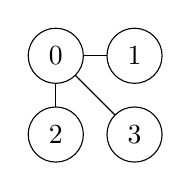
\begin{tikzpicture}
        \draw (0,1) -- (0,0);
        \draw (0,1) -- (1,0);
        \draw (0,1) -- (1,1);
        \foreach \x in {0,1} \foreach \y in {0,1}
            \draw (\x,\y) node[circle,draw,fill=white,inner sep=0,minimum size=0.7cm] {\pgfmathparse{int(2-2*\y+\x)}\pgfmathresult};
        \end{tikzpicture}
    \end{wrapfigure}
    Låt oss ta en titt på exemplet illustrerat till höger. I det här fallet så är alla
    korsningar bra startpositioner för polisen. Om hon startar i korsning $0$, så kan hon
    stå stilla under första draget och låta tjuven springa in i henne.
    Å andra sidan, om hon börjar i någon annan korsning så kan hon vänta tills tjuven
    når korsning $0$ och sedan flytta dit.

    Här är hur en exempel-session skulle kunna se ut:

    \begin{tabular}{|l|c|}
        \hline
            {\bf Funktionsanrop} & {\bf Returvärde} \\
        \hline
            \method{start(4, [[0, 1, 1, 1], [1, 0, 0, 0], [1, 0, 0, 0], [1, 0, 0, 0]])} &
            \constant{3} \\
        \hline
            \method{nextMove(1)} & \constant{3} \\
        \hline
            \method{nextMove(0)} & \constant{0} \\
        \hline
    \end{tabular}

    Anmärkning: i anropet till \method{start} ovanför så har \constant{true}
    och \constant{false} bytts ut mot \constant{1} och \constant{0} för att
    ta mindre plats.

    \Scoring

    \begin{description}
        \item[Deluppgift 1 (16 poäng):] $2 \le N \le 500$.
        För varje par av korsningar kommer det kommer att finnas exakt en väg som leder mellan dem.
        \item[Deluppgift 2 (14 poäng):] $2 \le N \le 500$. Nätverket av korsningar
        och gator kommer att bilda en rutnätsformad struktur. Rutnätet kommer att
        ha minst två rader och kolumner och korsningsnumreringen kommer att följa
        mönstret som illustreras i figuren nedan.
        \begin{figure}[h!]
           \centering
           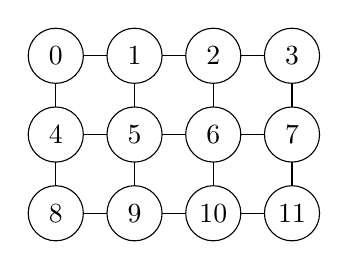
\begin{tikzpicture}
            \draw (0,0) grid (3,2);
            \foreach \x in {0,1,2,3} \foreach \y in {0,1,2}
                \draw (\x,\y) node[circle,draw,fill=white,inner sep=0,minimum size=0.7cm] {\pgfmathparse{int(8-4*\y+\x)}\pgfmathresult};
           \end{tikzpicture}
        \end{figure}
        \item[Deluppgift 3 (30 poäng):] $2 \le N \le 100$.
        \item[Deluppgift 4 (40 poäng):] $2 \le N \le 500$.
    \end{description}
    
    Din lösning skall uppfylla två krav:
    \begin{enumerate}
        \item korrekt bestämma huruvida polisen kan fånga tjuven;
        \item om detta är möjligt, fånga tjuven genom att göra drag
            åt polisen.
    \end{enumerate}
    
    I deluppgifter 1 och 2 så måste din lösning uppfylla båda kraven för att få några poäng.
    I deluppgifter 3 och 4 så kommer lösningar som bara implementerar det första kravet
    att få 30\% av deluppgiftens poäng. Om din lösning enbart satser på delpoäng så kan du
    terminera programmet genom att utföra vilket ogiltigt drag som helst (t.ex. kan du
    returnera $-1$ från \method{nextMove}).

    Notera att standardkraven (tids- och minnesgränser, inga körtidsfel) fortfarande
    måste uppfyllas för att få några poäng.
    \Constraints
    
    \begin{description}
        \item[Tidsgräns:] 1.5 s.
        \item[Minnesgräns:] 256 MB.
    \end{description}

    \Experimentation
    Exempelgradern på din dator kommer att läsa data från standard input.
    Första raden av indata ska innehålla ett heltal $N$ --- antalet korsningar.
    Följande $N$ rader ska innehålla närhetsmatrisen $A$. Varje rad ska
    innehålla $N$ tal, vardera antingen 0 eller 1. Matrisen måste vara
    symmetrisk, och värdena på huvuddiagonalen måste alla vara nollor.

    Nästa rad ska innehålla talet 1 om polisen kan fånga tjuven, och 0 annars.

    Till slut, om polisen kan fånga rånaren, ska det följa $N$ rader, som beskriver
    tjuvens flyktstrategi. Varje rad ska innehålla $N+1$ heltal mellan 0 och $N-1$.
    Värdet på rad $r$ och kolumn $c$, där $c < N$, motsvarar en situation där det
    är tjuvens tur, polisen befinner sig vid korsning $r$ och tjuven vid korsning $c$,
    och representerar korsningen som tjuven då ska röra sig till. Värdena på
    huvuddiagonalen kommer att ignoreras, då de motsvarar situationer då polis
    och tjuv befinner sig i samma korsning. Det sista värdet på rad $r$ beskriver
    tjuvens startkorsning om polisen startar i korsning $r$.
    
    Här är exempeldata till exempelgradern som representerar tre sammankopplade
    korsningar:

    \begin{center}
        \begin{tabular}{p{4cm}}
            {\tt
                3 \newline
                0 1 1 \newline
                1 0 1 \newline
                1 1 0 \newline
                1 \newline
                0 2 1 2 \newline
                2 0 0 2 \newline
                1 0 0 1 \newline
            }
        \end{tabular}
    \end{center}

    Och här är indatat som matchar exemplet givet ovan i problembeskrivningen:

    \begin{center}
        \begin{tabular}{p{4cm}}
            {\tt
                4 \newline
                0 1 1 1 \newline
                1 0 0 0 \newline
                1 0 0 0 \newline
                1 0 0 0 \newline
                1 \newline
                0 0 0 0 1 \newline
                2 0 0 0 2 \newline
                3 0 0 0 3 \newline
                1 0 0 0 1 \newline
            }
        \end{tabular}
    \end{center}
\end{document}
